\subsection{Begriffe}
Georg Cantor (1845-1918)
\begin{description}
    \item[Cantors naive Mengendefinition] Unter einer Menge verstehen wir eine Zusammenfassung von wohldefinierten Objekten $m$ unserer Anschauung oder unseres Denkens welche die Elemente von $M$ genannt werden, zu einem einheitlichen Ganzen.
    \item[Schreibweise]\
    \begin{itemize}
        \item $m \in M$ ($m$ ist Element von $M$)
        \item $m \not\in M$ ($m$ ist nicht Element von $M$, $\neg\ m \in M$)
    \end{itemize}
    \item[Mengendarstellung] verschiedene Möglichkeiten:
    \begin{itemize}
        \item allgemein mitels Eigenschaft $E(m)$ (Aussageform) $A=\lbrace m|E(m) \rbrace$ bzw.
        $$A = \lbrace m \in M | E(m) \rbrace = \lbrace m | m \in M \wedge E(m) \rbrace$$
        \item explizit für Menge mit wenigen endlich vielen Elementen:
        $$A=\lbrace a, b, c\rbrace$$
    \end{itemize}
    \item[Problem] Man darf nicht alle möglichen Zusammenfassungen bilden. Z.B.: die Menge aller Mengen die sich nicht selbst enthalten:
    $$R=\lbrace M | M \not \in M \rbrace$$
    $$R \in R \Leftrightarrow R \not \in R \equiv \bot$$
    \item[Lösung] Axiomatischer Aufbau der Mengenlehre
    \begin{description}
        \item[Extensionalitätsaxiom] Zwei Mengen A und B sind genau dann gleich, wenn sie die selben Elemente haben:
        $$A = B \Leftrightarrow (\forall x)(x \in A \Leftrightarrow x \in B)$$
        \item[Leere Menge] $\emptyset = \lbrace x | x \not = x\rbrace = \lbrace\rbrace$
        \item[Einermenge] $A=\lbrace a \rbrace$, $A = \lbrace x | x = a \rbrace$, $A \not = a$
        \item[Zweiermenge] $A=\lbrace a; b \rbrace$, $A = \lbrace x|(x=a \vee x=b) \wedge a \not = b \rbrace$
        \item[andere Mengen] \
        \begin{itemize}
            \item $\mathbb{N} = \lbrace 0;1;2;3;\dots \rbrace$ natürliche Zahlen
            \item $\mathbb{Z} = \lbrace \dots; (-1);0;1;\dots \rbrace$ ganze Zahlen
            \item $\mathbb{Q}$ rationale Zahlen
            \item $\mathbb{R}$ reelle Zahlen
            \item $\mathbb{C}$ komplexe Zahlen
        \end{itemize}
    \end{description}
    \item[Betrag] Anzahl der Elemente in der Menge (bei endlichen Mengen)
    \item[Teilmenge] $A \subseteq B \Leftrightarrow (\forall x)(x \in A \Rightarrow x \in B)$
    $$A \subseteq B \wedge B \subseteq C \Rightarrow A \subseteq C$$
    $$A \subseteq B \wedge B \subseteq A \Rightarrow A = B$$
    \item[Echte Teilmenge] $A \subset B$ oder $A \subsetneqq B \Leftrightarrow (\forall x)(x \in A \Rightarrow x \in B) \wedge A \not = B $
    \item[disjunkt] Die Mengen $A$ und $B$ heißen disjunkt (elementfremd) wenn: $A \cap B = \emptyset$
    \item[Kardinalität] Mächtigkeit
    \begin{description}
        \item[gleichmächtig] Zwei Mengen $A;B$ heißen gleich mächtig, wenn es eine bijektive Funktion $f : A \longrightarrow B$ gibt.
        $$A \sim B \Leftrightarrow (\exists f : A \longrightarrow B)$$
        $$A \sim B \wedge B \sim C \Rightarrow A \sim C$$
        \item[endlich] Menge $A$ heißt endlich, wenn $|A| \in \mathbb{N}$
        \item[abzählbar unendlich ] Eine Menge $A$ heißt abzählbar unendlich, wenn $$\mathbb{N} \sim A \wedge \exists f : \mathbb{N} \longrightarrow A\ \textrm{(bijektiv)}$$
        \item[nicht abzählbar unendlich] Meine Menge heißt nicht abzählbar unendlich, wenn sie weder endlich noch abzählbar unendlich ist.
        \item[Potenzmengen]$M \not \sim \mathcal{P}(M)$\\ Beweis:
        Angenommen es gäbe eine bijektive Funktion $f : A \longrightarrow \mathcal{P}(M)$ und
        $$A = \lbrace x \in M | x \not \in f(x) \rbrace \subset M$$
        Wir nehmen an dass $(\exists x \in M)\ f(x) = A$
        \begin{itemize}
            \item wenn $x \in f(x) $ dann $x \not \in A$ wegen $x \not \in f(x)$. Widerspruch da: $x \not \in A = x \not \in f(x)$
            \item wenn $x \not \in f(x)$ dann $x \in A$ wegen $x \in M$. Widerspruch da: $x \not \in A = x \not \in f(x)$
        \end{itemize}
    \end{description}
\end{description}
\subsection{Operationen auf Mengen}
\begin{description}
    \item[Vereinigung] $A \cup B = \lbrace x | x \in A \vee x \in B \rbrace$ \\
    \begin{tabular}{l|l|l}
        \adjustbox{valign = t}{
            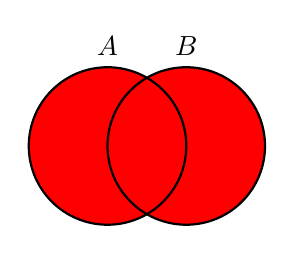
\begin{tikzpicture}[thick, set/.style = {circle, minimum size = 2cm, fill=red}]
                \node [set, label={90:$A$}] (A) at (-0.5,0) {};
                \node [set, label={90:$B$}] (B) at (0.5,0) {};
                \draw (-0.5,0) circle(1);
                \draw (0.5,0) circle(1);
            \end{tikzpicture}
        }                                                               &
        \adjustbox{valign = t}{
            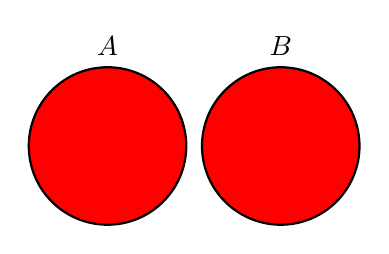
\begin{tikzpicture}[thick, set/.style = {circle, minimum size = 2cm, draw = black, fill=red}]
                \node [set, label={90:$A$}] (A) at (-1.1,0) {};
                \node [set, label={90:$B$}] (B) at (1.1,0) {};
            \end{tikzpicture}} &
        $\begin{array}{r c l}
             |A \cup B| & = & |A| + |B \setminus A| \\
             & = & |B| + |A \setminus B|
        \end{array}$
    \end{tabular}
    \item[Durchschnitt] $A \cap B := \lbrace x | x \in A \wedge x \in B \rbrace$ \\
    \begin{tabular}{l|l|l}
        \adjustbox{valign = t}{
            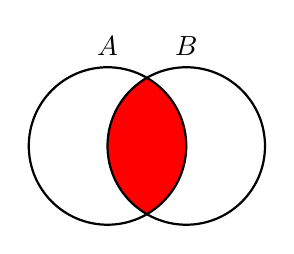
\begin{tikzpicture}[thick, set/.style = {circle, minimum size = 2cm, draw = black}]
                \begin{scope}
                    \clip (-0.5,0) circle(1);
                    \fill[red] (0.5, 0) circle (1);
                \end{scope}
                \node [set, label={90:$A$}] (A) at (-0.5,0) {};
                \node [set, label={90:$B$}] (B) at (0.5,0) {};
            \end{tikzpicture}
        } &
        \adjustbox{valign = t}{
            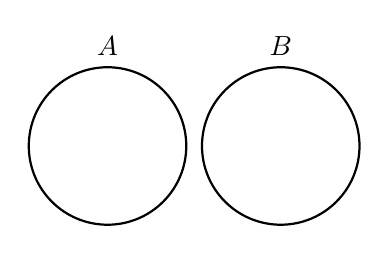
\begin{tikzpicture}[thick, set/.style = {circle, minimum size = 2cm, draw = black}]
                \node [set, label={90:$A$}] (A) at (-1.1,0) {};
                \node [set, label={90:$B$}] (B) at (1.1,0) {};
            \end{tikzpicture}
        } &
        $\begin{array}{r c l}
             |A \cap B| & = & |A| - |A \setminus B| \\
             & = & |B| - |B \setminus A|
        \end{array}$
    \end{tabular}
    \item[Mengendifferenz] $A \setminus B = \lbrace x | x \in A \wedge x \not \in B \rbrace$ \\
    \begin{tabular}{l|l|l}
        \adjustbox{valign = t}{
            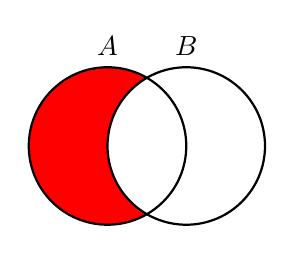
\begin{tikzpicture}[thick, set/.style = {circle, minimum size = 2cm, draw = black}]
                \begin{scope} [even odd rule]
                    \clip (-0.5,0) circle(1) (0.5,0) circle(1);1
                    \fill [red] (-0.5,0) circle (1);
                \end{scope}
                \node [set, label={90:$A$}] (A) at (-0.5,0) {};
                \node [set, label={90:$B$}] (B) at (0.5,0) {};
            \end{tikzpicture}
        } &
        \adjustbox{valign = t}{
            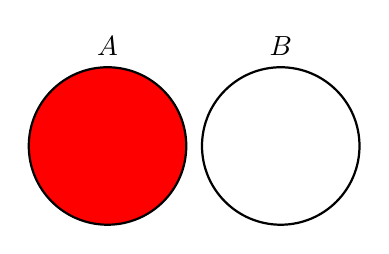
\begin{tikzpicture}[baseline=(current bounding box.north), thick, set/.style = {circle, minimum size = 2cm, draw = black}]
            \node [set, fill = red, label={90:$A$}] (A) at (-1.1,0) {};
            \node [set, label={90:$B$}] (B) at (1.1,0) {};
            \end{tikzpicture}
        } &
    \end{tabular}
    \item[symmetrische Differenz] $A \Delta B = (A \setminus B) \cup (B \setminus A)$ \\
    \begin{tabular}{l|l|l}
        \adjustbox{valign = t}{
            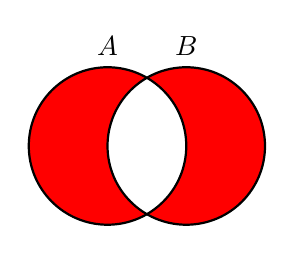
\begin{tikzpicture}[thick, set/.style = {circle, minimum size = 2cm, draw = black}]
                \fill [even odd rule, red] (-0.5,0) circle (1) (0.5,0) circle (1);
                \node [set, label={90:$A$}] (A) at (-0.5,0) {};
                \node [set, label={90:$B$}] (B) at (0.5,0) {};
            \end{tikzpicture}
        } &
        \adjustbox{valign = t}{
            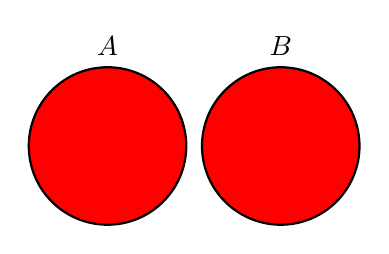
\begin{tikzpicture}[baseline=(current bounding box.north), thick, set/.style = {circle, minimum size = 2cm, draw = black, fill = red}]
            \node [set, label={90:$A$}] (A) at (-1.1,0) {};
            \node [set, label={90:$B$}] (B) at (1.1,0) {};
            \end{tikzpicture}
        } &
        $|A \Delta B| = |A \setminus B| + |B \setminus A|$
    \end{tabular}
    \item[Potenzmengen] $\mathcal{P}(A) \coloneqq \lbrace B|B \subseteq A \rbrace;\ |\mathcal{P}(A)| = 2^{|A|}$
    \item[ungeordnets Paar] $\lbrace a,b \rbrace = \lbrace c,d \rbrace \Rightarrow (a=c \wedge b=d) \vee (a=d \wedge b=c)$
    \item[geordnetes Paar] $\lbrace a,b \rbrace = \lbrace c,d \rbrace \Rightarrow a=c \wedge b=d$ (Das geht!)
    \item[Mengenprodukt] $A \times B = \lbrace (a,b)|a \in A \wedge b \in B \rbrace$ (nicht Kommutativ, (strenggenommen) nicht assoziativ)
    \begin{align*}
    (A \times B) \times C & \not = A \times (B \times C) \\
    ((a,b),c)             & \not = (a,(b,c))
    \end{align*}
    Gegeben sein
    $$A = \lbrace 1, 2 \rbrace$$
    $$B = \lbrace a, b, c \rbrace$$
    dann ist:
    $$A \times B = \lbrace (1,a),(2,a)(1,b)(2,b),(1,c)(2,c) \rbrace$$ \\
    $|A \times B| = |A| \cdot |B|$
\end{description}
